\documentclass[tikz,border=2pt]{standalone}
\usepackage{tikz}
\begin{document}
  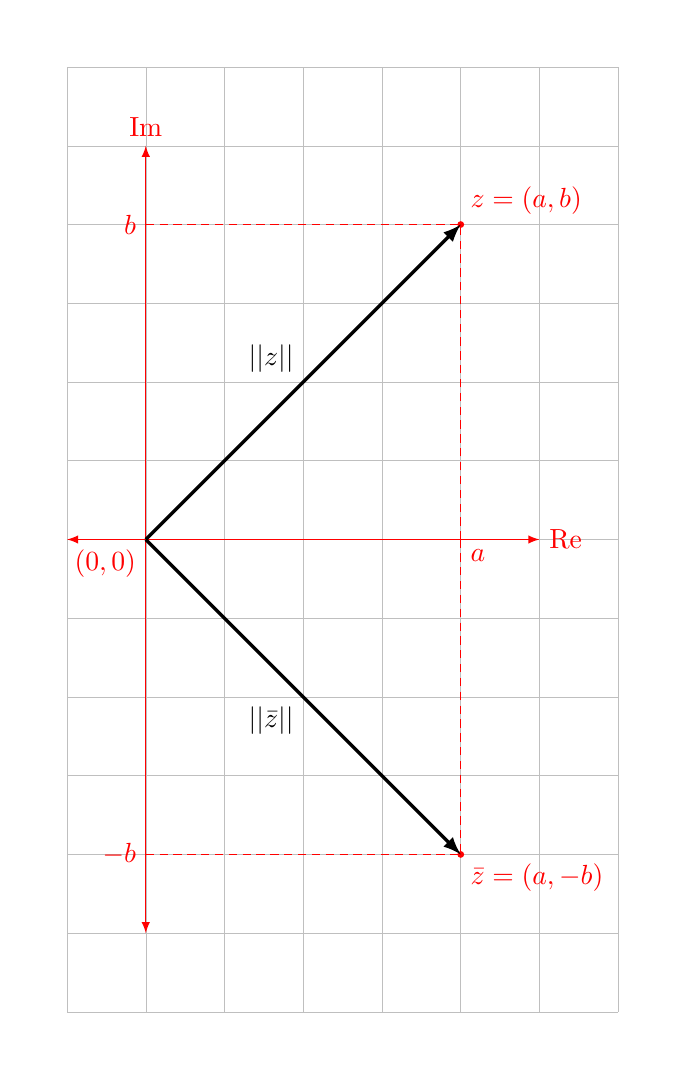
\begin{tikzpicture}
    \fill[white] (-1.5,-6.5) rectangle (6.5,6.5);
    \draw[lightgray,very thin] (-1,-6) grid (6,6);
    \draw (0,0) node[red,below left]{$(0,0)$};
    \draw[red,latex-latex] (-1,0) -- (5,0) node[right]{Re};
    \draw[red,latex-latex] (0,-5) -- (0,5) node[above]{Im};
    \filldraw[red] (4,4) circle(1pt) node[above right]{$z=(a,b)$};
    \filldraw[red] (4,-4) circle(1pt) node[below right]{$\bar{z}=(a,-b)$};
    \draw[very thick,-latex] (0,0) -- (4,4);
    \draw (4,0) node[red,below right]{$a$};
    \draw (0,4) node[red,left]{$b$};
    \draw[red,densely dashed] (4,0) -- (4,4);
    \draw[red,densely dashed] (0,4) -- (4,4);
    \draw (2,2) node[above left]{$||z||$};
    \draw[very thick,-latex] (0,0) -- (4,-4);
    \draw (0,-4) node[red,left]{$-b$};
    \draw[red,densely dashed] (4,0) -- (4,-4);
    \draw[red,densely dashed] (0,-4) -- (4,-4);
    \draw (2,-2) node[below left]{$||\bar{z}||$};
  \end{tikzpicture}
\end{document}
